\chapter{Конструкторский раздел}

В данном разделе будут спроектированы схемы алгоритмов, произведена оценка трудоемкости алгоритмов, описаны используемые типы данных, а также произведена оценка памяти и описана структура ПО.

\section{Схемы алгоритмов}

В следующих схемах матрица будет представлена как $A$, $B$ или $Res$, а $A_{i_j}$ - j-ый элемент i-ой строки матрицы $A$.

На рисунках 2.1 - 2.3 представлены схемы рассматриваемых алгоритмов.

В качестве оптимизаций алгоритма Винограда выбрано использование +=, использование переменной-буфера и проверка на нечетность внутри цикла.
 
\newpage
\begin{figure}[h!]
	\begin{center}
		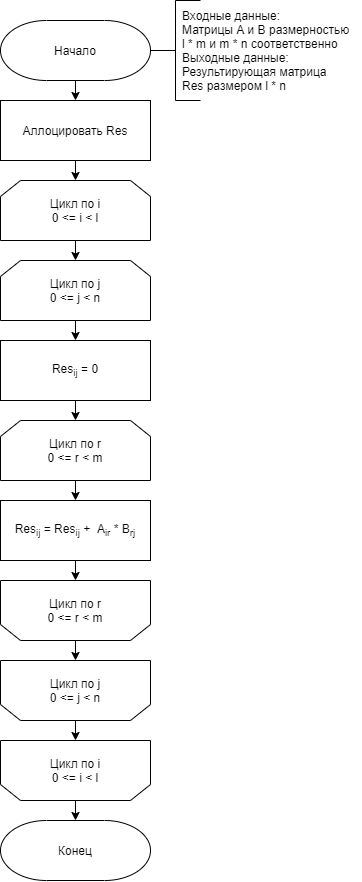
\includegraphics[scale=0.6]{assets/multStand.png}
	\end{center}
	\caption{Схема стандартного алгоритма умножения матриц}
\end{figure}

\newpage 
\begin{figure}[h!]
	\begin{center}
		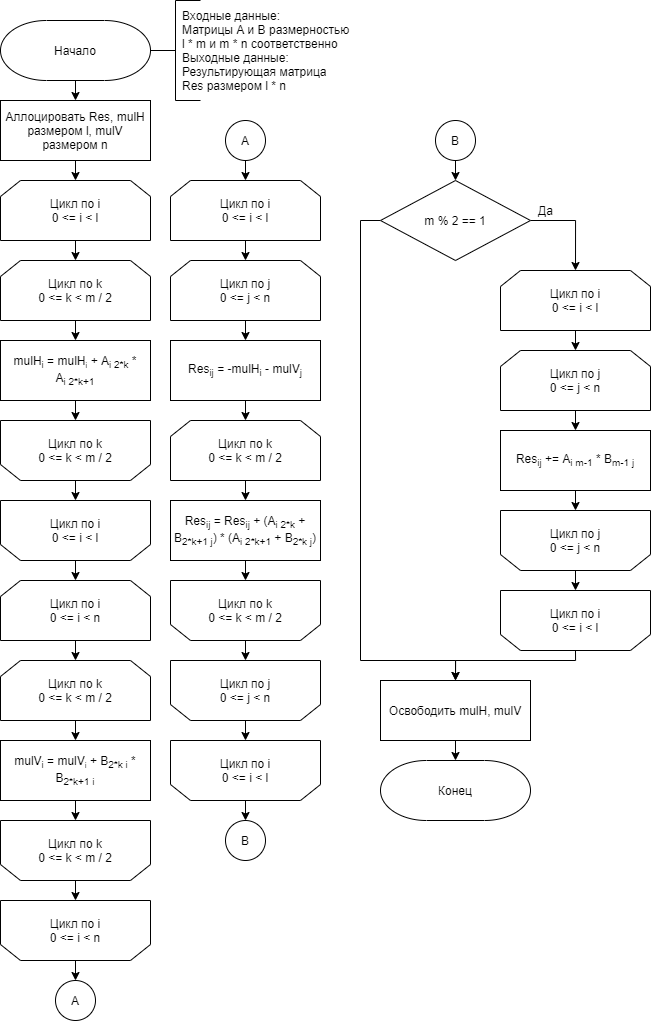
\includegraphics[scale=0.6]{assets/multVin.png}
	\end{center}
	\caption{Схема алгоритма умножения матриц Винограда}
\end{figure}

\newpage 
\begin{figure}[h!]
	\begin{center}
		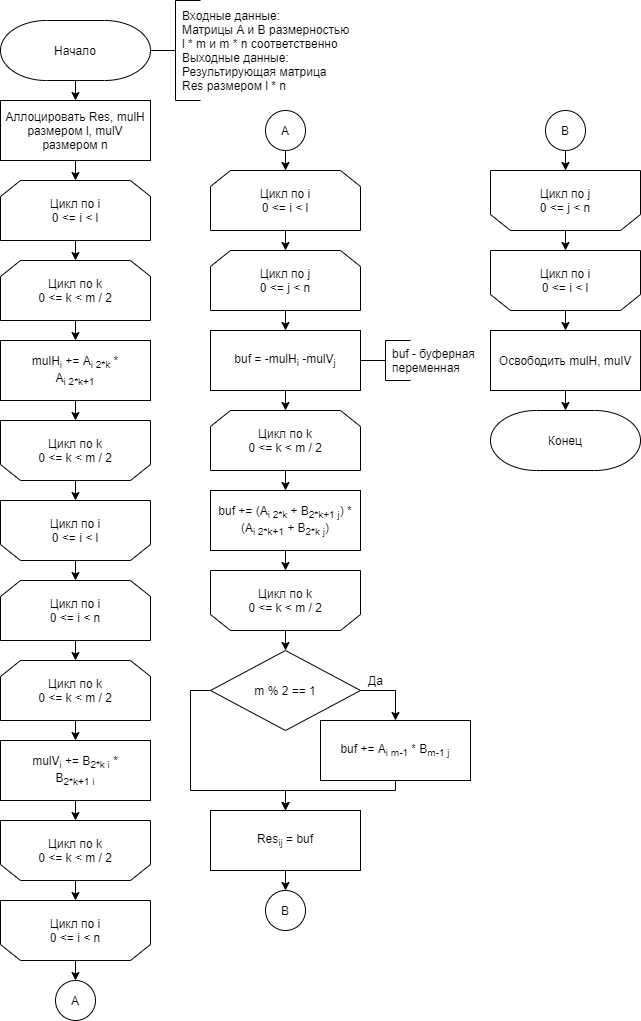
\includegraphics[scale=0.6]{assets/multVinOpt.png}
	\end{center}
	\caption{Схема алгоритма умножения матриц Винограда (оптимизированный)}
\end{figure}

\newpage
\section{Модель оценки трудоемкости алгоритмов}

\subsection{Трудоемкость алгоритмов}

Введем модель оценки трудоемкости.

\begin{enumerate}
	\item Трудоемкость базовых операций
		\begin{itemize}
			\item Примем трудоемкость следующих операций равной 1:
			\begin{equation}
				=, +, -, +=, -=, ==, !=, <, >, \leq, \geq, !, \&\&, ||, []
			\end{equation}
			\item Примем трудоемкость следующих операций равной 2:
			\begin{equation}
				*, /, \%, *=, /=,
			\end{equation}
		\end{itemize}
	\item Трудоемкость циклов
	\begin{equation}
		f = f_{init} + f_{compare} + N_{iter} * (f_{body} + f_{inc} + f_{compare})
	\end{equation}
	\item Трудоемкость условного оператора
		Пусть трудоемкость самого условного перехода равна 0. Тогда
		\begin{equation}
			f_{if} = f_{condition} + 
			\begin{sqcases}
				min(f_{true}, f_{false}), \text{в лучшем случае}\\
				max(f_{true}, f_{false}), \text{в худшем случае}\\				
			\end{sqcases}
		\end{equation}
\end{enumerate}

где \newline
$f_{init}$ - трудоемкость инициализации, \newline
$f_{compare}$ - трудоемкость сравнения, \newline
$N_{iter}$ - количество итераций, \newline
$f_{body}$ - трудоемкость тела цикла, \newline
$f_{inc}$ - трудоемкость инкрементации, \newline
$f_{condition}$ - трудоемкость условия, \newline
$f_{true}$, $f_{false}$ - трудоемкость веток условного оператора.
\newpage

\subsection{Трудоемкость станадртного алгоритма}

Трудоемкость стандартного алгоритма сосоит из:
\begin{itemize}
	\item трудоемкость цикла по i от 1 до L: $f = 2 + L(2 + f_{body})$;
	\item трудоемкость цикла по j от 1 до N: $f = 2 + 3 + N(2 + f_{body})$;
	\item трудоемкость цикла по r от 1 до M: $f = 2 + M(2 + 12) = 2 + 14M$.
\end{itemize}

Итого, трудоемкость стандартного алгоритма равна:
\begin{equation}
    f = 2 + L(2 + 2 + N(2 + 3 + 2 + 14M)) = 2 + 4L + 7LN + 14LNM \approx 14LNM \approx O(N^3)
\end{equation}

\subsection{Трудоемкость алгоритма Винограда}

Трудоемкость алгоритма Винограда состоит из:
\begin{itemize}
    \item аллокация и инициализация векторов mulH и mulV: $f_{HV} = L + N + 2 + L(2 + 3 + \frac{1}{2}M(3 + 14)) + 2 + N(2 + 3 + \frac{1}{2}M(3 + 14)) = 2 + 6L + 6N + \frac{17}{2}LM + \frac{17}{2}NM$;
    \item цикл по i от 1 до L: $f_{L} = 2 + L(2 + f_{body})$;
    \item цикл по j от 1 до N: $f_{N} = 2 + N(2 + 7 + f_{body})$;
    \item цикл по k от 1 до M/2: $f_{M/2} = 3 + \frac{1}{2}M(3 + 28) = 3 + \frac{31}{2}M$;
    \item проверка размеров на нечетность:
    \begin{equation}
    	f_{if} = 3 + \begin{sqcases}
    			0, & \text{л.с.}\\
    			2 + L(2 + 2 + N(2 + 11)) & \text{х.с.}\\
    		\end{sqcases}
    \end{equation}
\end{itemize}

\newpage
Итого, трудоемкость алгоритма Винограда для лучшего случая равна:
\begin{equation}
	f = 4 + 10L + 6N + \frac{17}{2}LM + \frac{17}{2}NM + 12LN + \frac{31}{2}LNM \approx 15,5LNM \approx O(N^3)
\end{equation}

Для худшего случая равна:
\begin{equation}
	f = 6 + 14L + 6N + \frac{17}{2}LM + \frac{17}{2}NM + 25LN + \frac{31}{2}LNM \approx 15,5LNM \approx O(N^3)
\end{equation}

\subsection{Трудоемкость оптимизированного алгоритма Винограда}

Трудоемкость оптимизированного алгоритма Винограда состоит из:
\begin{itemize}
    \item аллокация и инициализация векторов mulH и mulV: $f_{HV} = L + N + 2 + L(2 + 3 + \frac{1}{2}M(3 + 13)) + 2 + N(2 + 3 + \frac{1}{2}M(3 + 13)) = 2 + 6L + 6N + 8LM + 8NM$;
    \item цикл по i от 1 до L: $f_{L} = 2 + L(2 + f_{body})$;
    \item цикл по j от 1 до N: $f_{N} = 2 + N(2 + 5 + f_{body} + f_{if} + 3)$;
    \item цикл по k от 1 до M/2: $f_{M/2} = 3 + \frac{1}{2}M(3 + 23) = 3 + 13M$;
    \item проверка размеров на нечетность:
    \begin{equation}
    	f_{if} = 3 + \begin{sqcases}
    			0, & \text{л.с.}\\
    			10 & \text{х.с.}\\
    		\end{sqcases}
    \end{equation}
\end{itemize} 

\newpage
Итого, трудоемкость оптимизированного алгоритма Винограда для лучшего случая равна:
\begin{equation}
	f = 4 + 10L + 6N + 8LM + 8NM + 16LN + 13LNM \approx 13LNM \approx O(N^3)
\end{equation}

Для худшего случая равна:
\begin{equation}
	f = 4 + 10L + 6N + 8LM + 8NM + 26LN + 13LNM \approx 13LNM \approx O(N^3)
\end{equation}

\section{Используемые типы данных}

При реализации алгоритмов будут использованы следующие структуры данных:
\begin{itemize}
	\item матрица типа int заданного размера;
	\item размеры матрицы - целое число int;
	\item вспомогательные массивы типа int заданного размера.
\end{itemize}

\section{Оценка памяти}

Пусть matrix - матрица целых чисел, l * m и m * n - размерность входных матриц и l * n - результирующей.

Для стандартного алгоритма умножения будет затрачена память на:
\begin{itemize}
	\item размеры матрицы - 3 * sizeof(int);
	\item матрицы - (l * m + m * n + l * n) * sizeof(int).
\end{itemize}

Для алгоритма Винограда создаются два дополнительных массива, для которых используется (l + n) * sizeof(int) памяти. Для оптимазации алгоритма используется вспомогательная переменная buf размером sizeof(int).

Станадартный алгоритм обходится без использования дополнительной памяти, что дает ему выигрыш, хоть и незначительный.

\section{Структура ПО}

ПО будет состоять из следующих модулей:
\begin{itemize}
	\item Главный модуль - из него будет осуществляться запуск программы и выбор соответствующего режима работы;
	\item Модуль интерфейса - в нем будет описана реализация режимов работы программы;
	\item Модуль, содержащий функции работы с данными (такие как генерация данных, вывод, обмен значениями);
	\item Модуль, содержащий реализации алгоритмов.
\end{itemize}

\section{Вывод}

На основе полученных в аналитическом разделе знаний об алгоритмах были спроектированы схемы алгоритмов, произведена оценка их трудоемкости, выбраны используемые типы данных, проведена оценка затрачиваемого объема памяти, а также описана структура ПО.